
\documentclass[conference]{IEEEtran}

\usepackage[pdftex]{graphicx}
\graphicspath{ {../images/} }
\usepackage{caption}
\usepackage{subcaption}
\usepackage{float}
\usepackage{amsmath}

\usepackage{hyperref}
\hypersetup
{
    colorlinks=true,
    linkcolor=black,   
    urlcolor=blue,
    citecolor=black,
}

\usepackage{pdfpages}
\renewcommand{\familydefault}{\sfdefault}

% *** ALIGNMENT PACKAGES ***
%
%\usepackage{array}
% Frank Mittelbach's and David Carlisle's array.sty patches and improves
% the standard LaTeX2e array and tabular environments to provide better
% appearance and additional user controls. As the default LaTeX2e table
% generation code is lacking to the point of almost being broken with
% respect to the quality of the end results, all users are strongly
% advised to use an enhanced (at the very least that provided by array.sty)
% set of table tools. array.sty is already installed on most systems. The
% latest version and documentation can be obtained at:
% http://www.ctan.org/tex-archive/macros/latex/required/tools/


%\usepackage{mdwmath}
%\usepackage{mdwtab}
% Also highly recommended is Mark Wooding's extremely powerful MDW tools,
% especially mdwmath.sty and mdwtab.sty which are used to format equations
% and tables, respectively. The MDWtools set is already installed on most
% LaTeX systems. The lastest version and documentation is available at:
% http://www.ctan.org/tex-archive/macros/latex/contrib/mdwtools/


% IEEEtran contains the IEEEeqnarray family of commands that can be used to
% generate multiline equations as well as matrices, tables, etc., of high
% quality.


% *** SUBFIGURE PACKAGES ***
%\usepackage[tight,footnotesize]{subfigure}
% subfigure.sty was written by Steven Douglas Cochran. This package makes it
% easy to put subfigures in your figures. e.g., "Figure 1a and 1b". For IEEE
% work, it is a good idea to load it with the tight package option to reduce
% the amount of white space around the subfigures. subfigure.sty is already
% installed on most LaTeX systems. The latest version and documentation can
% be obtained at:
% http://www.ctan.org/tex-archive/obsolete/macros/latex/contrib/subfigure/
% subfigure.sty has been superceeded by subfig.sty.


% *** FLOAT PACKAGES ***
%
%\usepackage{fixltx2e}
% fixltx2e, the successor to the earlier fix2col.sty, was written by
% Frank Mittelbach and David Carlisle. This package corrects a few problems
% in the LaTeX2e kernel, the most notable of which is that in current
% LaTeX2e releases, the ordering of single and double column floats is not
% guaranteed to be preserved. Thus, an unpatched LaTeX2e can allow a
% single column figure to be placed prior to an earlier double column
% figure. The latest version and documentation can be found at:
% http://www.ctan.org/tex-archive/macros/latex/base/



\usepackage{stfloats}
% stfloats.sty was written by Sigitas Tolusis. This package gives LaTeX2e
% the ability to do double column floats at the bottom of the page as well
% as the top. (e.g., "\begin{figure*}[!b]" is not normally possible in
% LaTeX2e). It also provides a command:
%\fnbelowfloat
% to enable the placement of footnotes below bottom floats (the standard
% LaTeX2e kernel puts them above bottom floats). This is an invasive package
% which rewrites many portions of the LaTeX2e float routines. It may not work
% with other packages that modify the LaTeX2e float routines. The latest
% version and documentation can be obtained at:
% http://www.ctan.org/tex-archive/macros/latex/contrib/sttools/
% Documentation is contained in the stfloats.sty comments as well as in the
% presfull.pdf file. Do not use the stfloats baselinefloat ability as IEEE
% does not allow \baselineskip to stretch. Authors submitting work to the
% IEEE should note that IEEE rarely uses double column equations and
% that authors should try to avoid such use. Do not be tempted to use the
% cuted.sty or midfloat.sty packages (also by Sigitas Tolusis) as IEEE does
% not format its papers in such ways.

% correct bad hyphenation here
\hyphenation{op-tical net-works semi-conduc-tor}

%\usepackage[style=numeric,sorting=none]{biblatex}
\usepackage[backend = bibtex,style=numeric,sorting=none]{biblatex}
\addbibresource{AINT308.bib}

\usepackage{amsmath}

\begin{document}
%
% paper title
% can use linebreaks \\ within to get better formatting as desired
\title{AINT308 - Machine Vision and Behavioural Computing\\Coursework 2 Report}


% author names and affiliations
% use a multiple column layout for up to three different
% affiliations
\author{\IEEEauthorblockN{Student No. 10613591}
\IEEEauthorblockA{School of Engineering,\\Computing and Mathematics
\\University of Plymouth\\
Plymouth, Devon}}



% make the title area
\maketitle


\begin{abstract}
%\boldmath
 Machine Vision is a field of study whose applications are becoming rapidly more prevalent amongst contemporary technology, with advancements having considerable implications in various fields. This report details the use of a popular open-source machine vision library, \textbf{OpenCV}, in two additional real-world applications: Using disparity mapping to estimate the distance to an object, and using edge detection to detect road markings.
\end{abstract}
\subsection*{Keywords:}
Machine Vision, OpenCV, Object Tracking, C++

\section{Task 4 - Disparity Mapping}
\textit{For accompanying large figures, see appendix \ref{app:T4}}

\textit{For the video demo, click \href{https://youtu.be/kQwU62_2fdQ}{HERE}}
\subsection{Introduction}
This task demonstrates the use of disparity maps in order to estimate the distance from a stereo vision system to an object.
\subsection{Solution}
An important first step when working with stereo visions systems is to account for distortions in the image. A number of factors, including both distortions caused by the camera itself as well as distortions caused by a human element of the camera's operation, can induce this\cite{Distortions}.

Without properly calibrating, these distortions and inaccuracies can have a catastrophic effect on the ability for the system to function. This is even more important for applications with safety-critical consequences, such as vision systems for self-driving cars\cite{Bosch} or industrial monitoring equipment\cite{Intel}.

There are multiple methods for performing the calibration. MATLAB's implementation uses Bouguet's method\cite{MATLAB_Calibration}\cite{Bouguet}, whereas Hartley's method\cite{hartley2003multiple} also exists as an alternative. \textit{OpenCV's} built-in calibration function can use both algorithms\cite{Book_Calibration}.

The calibration function uses pairs of chequerboard images and generates sets of \textit{intrinsic} and \textit{extrinsic} parameters. The \textit{intrinsic} parameters contain the focal length, principal point, and skew coefficient, all of which are distortion sources local to the camera. The extrinsic parameters store the rotation and translation between the two cameras. 

The generated calibration data is loaded into the program, and used to distort the images to correct the distortion created. With perfect calibration, the two distortions will completely cancel out, leaving a perfect fidelity image. \textit{OpenCV's} \verb|remap|\cite{remap} function is used to perform the correct. The \verb|remap| function takes in an input array as well as up to two maps to perform the re-mapping, in this case, the input image and the two generated maps created using the intrinsic and extrinsic parameters, outputting the results to a destination array\cite{remap_docs}.

The disparity is used to estimate the distance to an object from the camera. By using the parallax of the two stereo cameras combined with the disparity mapping, the approximate distance of the object can be triangulated. This is similar to how the human brain estimates distance using \textit{binocular disparity}\cite{10.3389/fpsyg.2014.00870}\cite{BERRYHILL2012525} and is another example of how robotics emulates life to mimic functionality. Astronomers use similar techniques to measure the distance to stellar objects\cite{parallax}.

Semi-Global Block Matching (SGBM) is used to generate a disparity map. SGBM takes a small region in one image, and searches in nearby locations in the other image for matches. The disparity is the minimum distance needed to find a match. Sum of Absolute Differences (SAD) is used to calculate the similarity\cite{StereoBlockMatching}. The value of each pixel in the template section is subtracted from the respective pixel in the target section, then these differences are summed. The lower the value, the closer the match. It should be noted that before this operation, the images are converted to grey scale, to minimise the amount of data needed to be processed, as each pixel can be represented as a single 8-bit value.

\begin{equation} \label{eq:disparity}
Disparity = \frac{B \bullet f}{Distance}
\end{equation}
\begin{equation} \label{eq:BF}
B \bullet f = Distance \bullet Disparity
\end{equation}
\begin{equation}	\label{eq:Distance}
Distance = \frac{B\bullet f}{Disparity}
\end{equation}

To use the \textit{Disparity-Distance} formula, the unknown parameter $B \bullet f$ needed to be derived using the supplied known distances. The pixel $(280,350)$ was chosen as the approximate centre of the target in the known distance images, and it's intensity extracted. To reduce the likelihood of errors, an average of the 3x3 grid around this point was taken. The results can be seen in Table \ref{tab:intensity_results}. Using equations \ref{eq:disparity} and \ref{eq:BF}, it is possible to approximate the value of $B \bullet f = 62426$. Derivation of the values of $B$ and $f$ individually is not necessary for the task. 

Table \ref{tab:t4_partial} shows the error results at different distances, with the maximum error being a 3.11\%. This is within the 5\% margin of error expected of the system.

To make the guesses on the distance to the target in the unknown image, the same process is repeated. The unknown image pairs are read in, and are grey-scaled before using SGBM to produce a disparity map. The retrieved average intensity is used in Equation \ref{eq:Distance} to produce an estimate for the distance to the target. The results can be seen in Table \ref{tab:t4_guesses}. 

\begin{table}[]
\caption{Intensity Readings At Known Distances}
\label{tab:intensity_results}
\begin{tabular}{|l|l|l|}
\hline
\textbf{Distance} & \textbf{Single Pixel Avg} & \textbf{3x3 Avg} \\ \hline
30                 & 2094 & 2093         \\ \hline
40                & 1566 & 1565         \\ \hline
50                 & 1245 & 1245         \\ \hline
60                 & 1040 & 1040         \\ \hline
70                 & 896 & 896         \\ \hline
80                & 784 & 783         \\ \hline
90                & 703 & 703         \\ \hline
100                 & 632 & 631          \\ \hline
110      & 576 & 576           \\ \hline
120      & 514 & 513         \\ \hline
130                 & 480 &479          \\ \hline
140				& 432	& 432	\\ \hline
150				&	414 & 414	\\ \hline
\end{tabular}
\end{table} 

\begin{table}[]
\caption{Program results and error rate}
\label{tab:t4_partial}
\begin{tabular}{|l|l|l|}
\hline
\textbf{Distance} & \textbf{Program Result} & \textbf{Program Error} \\ \hline
30                & 29.8134                 & 0.62\%                 \\ \hline
40                & 39.8747                 & 0.31\%                 \\ \hline
50                & 50.1235                 & -0.25\%                \\ \hline
60                & 60.025                  & -0.04\%                \\ \hline
70                & 69.6632                 & 0.48\%                 \\ \hline
80                & 79.6928                 & 0.38\%                 \\ \hline
90                & 88.7714                 & 1.37\%                 \\ \hline
100               & 98.8448                 & 1.16\%                 \\ \hline
110               & 108.378                 & 1.47\%                 \\ \hline
120               & 121.556                 & -1.30\%                \\ \hline
130               & 130.175                 & -0.13\%                \\ \hline
140               & 144.356                 & -3.11\%                \\ \hline
150               & 150.747                 & -0.50\%                \\	\hline
\end{tabular}
\end{table}

\begin{table}[]
\caption{Distance estimates for unknown image pairs}
\label{tab:t4_guesses}
\begin{tabular}{|l|l|}
\hline
\multicolumn{1}{|l|}{\textbf{Image \#}} & \textbf{Distance Value} \\	\hline
0                                       & 105.193                 \\	\hline
1                                       & 59.1529                 \\	\hline
2                                       & 114.754                 \\	\hline
3                                       & 151.847                 \\	\hline
4                                       & 49.4572                 \\	\hline
5                                       & 134.862                 \\	\hline
6                                       & 28.9247                 \\	\hline
7                                       & 83.3458                 \\	\hline
\end{tabular}
\end{table}
%\begin{figure}[H]
%\centering
%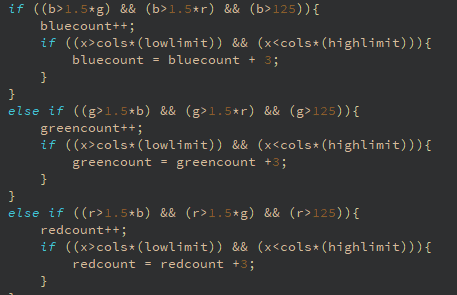
\includegraphics[width=2.5in]{t1}
%\caption{Pixel testing code}
%\label{fig_t1code}
%\end{figure}

\subsection{Limitations}
Given that the system displayed accurate results with the known dataset, and that without the true distances of the unknown dataset performance cannot be conclusively verified, the system performed to specifications. It is difficult to identify limitations given the limited scope of testing, and lack of access to additional testing materials.

\subsection{Further Improvements} \label{sec:further1}
 This system's performance is directly tied to the quality of it's calibration, so more accurate calibration data would benefit it's performance. This could be done by having less clutter in the calibration images. Ideally, they would be shot on a plain background, with the only difference being the target moving. Additionally, the distance of the target could be measured with a more accurate and precise instrument, to further ensure the quality of the calibration.
 
One disadvantage of using SGBM is that it is very processing intensive, especially as the size of the area to be searched increases. Performing SGBM on larger images on less powerful hardware may not be possible in real-time. To alleviate this, Field Programmable Gate Arrays (FPGAs) can be used to create bespoke hardware capable of performing the SGBM at high speeds\cite{HardwareSGBM}.
\subsection{Conclusion}
The system performed extremely well, correctly identifying every target distance with a sub 5\% error rate. It can be said that the task was a success, despite not knowing the performance when estimating the unknown targets, due to the performance with the testing targets. This demonstrates that disparity and parallax can be used to calculate distance to a target using a simple software solution, and \textit{OpenCV}. 

\section{Task 5 - Lane Tracking}
\textit{For accompanying large figures, see appendix \ref{app:T5}}

\textit{For the video demo, click \href{https://youtu.be/kW5fbNTTovo}{HERE}}

The second task involves using edge detection to correctly identify the current lane in a piece of dashboard camera footage. 
\subsection{Introduction}
Giving computers the ability to recognise lines has many potential applications, one of the foremost being for self-driving cars and other related applications. Edge detection is one method of letting computers recognise lines, and in this application will be used to recognise lane demarcations on roads, using dashboard camera footage as a testing medium.
\subsection{Solution}\label{2_solution}
After loading in a frame of video data, \textit{OpenCV's} \verb|cvtColour| function is used, to convert the image to greyscale. For this implementation, colour information is not necessary, and while it's loss does reduce the efficacy of edge-detection \cite{GreyVSColor}, the solution still performed adequately.  

When performing edge detection, it is important to apply filtering to smooth the image, and remove noise. Noise may cause contiguous edges to be picked up as many, smaller edges.  To do this, \textit{OpenCV's} \verb|blur| function is used. At it's default settings, \verb|blur| employs a variable sized normalized box filter to smooth an image\cite{BlurDocs}. $3$x$3$ was chosen, too large a kernel and the more granular details of the image would be lost, whereas too small a kernel would mean the smoothing had very little effect on the image.

During operation, the edge detection would detect false positives in the tree line. This effect is unavoidable, no matter what parameters for the edge detection are used. To avoid this, a rectangular overlay is added to the video feed, blocking the top half of the video. This overlay prevents the upper half of the image from going though the edge detection algorithm, and consequently stops false-positives in the tree-line from being detected.

The solution uses Canny edge detection in order to detect the lines within the target image. \textit{OpenCV} implements Canny edge detection using the \verb|Canny| function\cite{8265710}, which takes in an input and output frame as well as an upper and lower threshold, \verb|upperThreshold| and \verb|lowerThreshold|. Figure \ref{fig:Canny} shows the output of Canny edge detection on an example video frame. Changing the threshold values changes the sensitivity of the edge detection. The final values chosen in the solution are $50$ and $100$. Different values were experimented with, however the main factor that changed the performance of the solution was the Hough Lines parameters, discussed below. 

\begin{figure}[H]
\centering
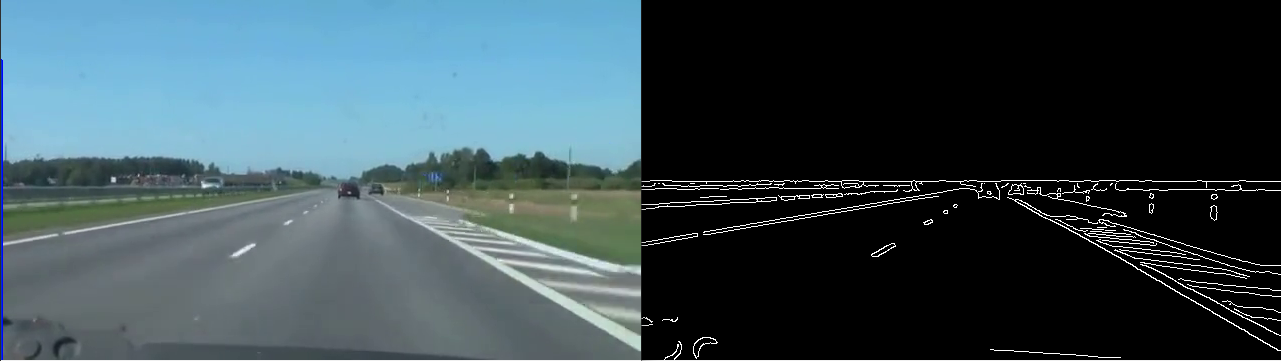
\includegraphics[width=3.5in]{t5_edge}
\caption{Example of Canny edge detection}
\label{fig:Canny}
\end{figure}
 

A Hough Lines transform can be used to detect straight lines. The \textit{OpenCV} implementation allows for two different variations, a \textit{Standard Hough Lines Transform} and a \textit{Probabilistic Hough Lines Transform}. The standard transform allows for detection of straight lines and is highly resistant to noise \cite{4608701}. The probabilistic transform is more efficient, as it only calculates part of the transform, and is able to handle curved lines and segmented lines better. However, it is less resistant to noise, and with the limited pre-processing performed worse than its standard counterpart. See Figure \ref{fig:houghComp} for a comparison between the two variations with no pre-processing. 
\begin{figure}[H]
\centering
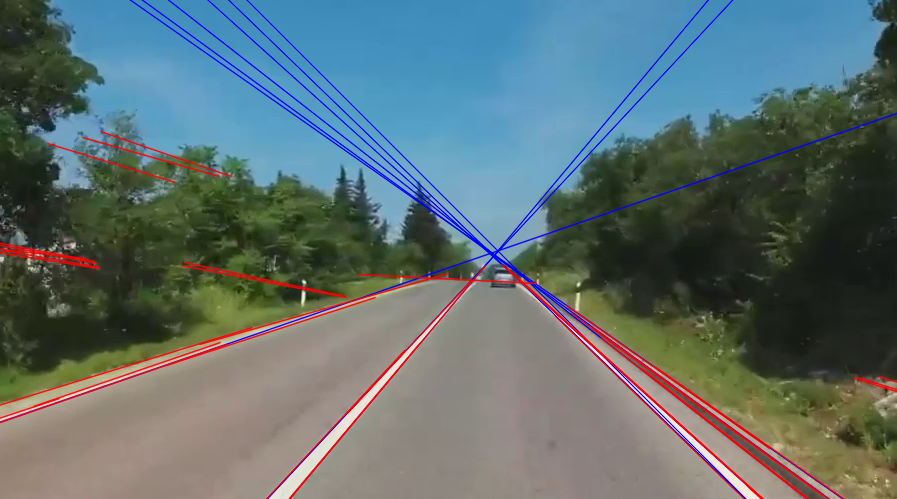
\includegraphics[width=3.5in]{t5_houghcomp}
\caption{Comparison of Hough Transform variants, standard in blue, probabilistic in red}
\label{fig:houghComp}
\end{figure}
\begin{figure}[H]
\centering
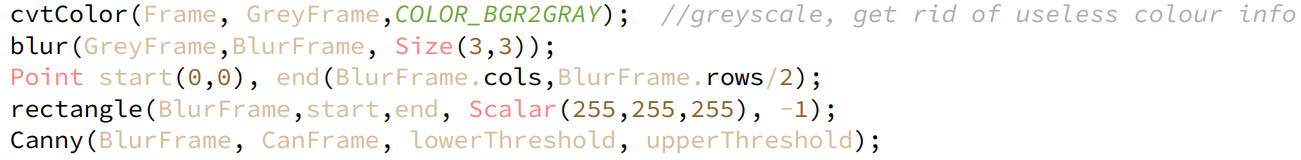
\includegraphics[width=3.5in]{t5_proc}
\caption{Pre-processing code}
\label{fig:t5proc}
\end{figure}
With the vector of lines detected by the Hough Transform, rendering can begin. The solution makes use of \textit{Temporal Smoothing}\cite{TemporalSmoothing} in order to reduce the amount of jitter between frames. Jitter means the displayed lane boundaries would jump, which is undesirable behaviour and could have negative effects towards the safety of the end user. Temporal Smoothing works by checking the new (current frame) coordinates against the old (previous frame) coordinates. If the change is greater than the threshold, then it is reduced to 10\% of the difference, and then the line is rendered. This greatly reduces the amount of jitter, improving the quality of the lane detection. 

Equations \ref{eq:line} and \ref{eq:line_para} are both equations that represent lines, non-parametric and parametric respectively. In the parametric equation, $\rho$ represents the perpendicular distance from the line to the origin, and $\theta$ is the angle between the perpendicular and the horizontal axis, measured counter-clockwise\cite{HoughRT}. Representing lines parametrically avoids undefined computational behaviour present in the standard model when lines are completely vertical or horizontal. 
\begin{equation}\label{eq:line}
y = mx + c
\end{equation}
\begin{equation}\label{eq:line_para}
\rho = x \cos\theta + y \cos\theta
\end{equation}

\begin{figure}[H]
\centering
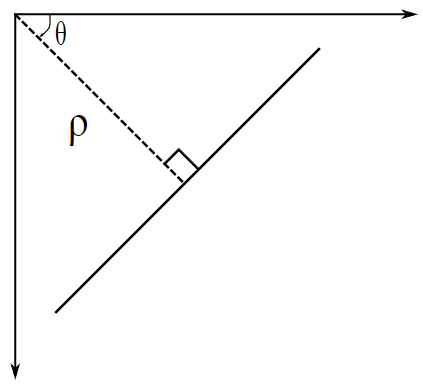
\includegraphics[width=2.5in]{t5_rhotheta}
\caption{Parametric representation of lines\cite{HoughRT}}
\label{fig:t5proc}
\end{figure}

The solution only renders lines that meet one of the following constraints: \begin{itemize}
\item[] $\rho \leq 1$ \textbf{OR} $\rho \geq 2.3$
\end{itemize} This only renders lines that fall close to the vertical, of which the majority of the lane demarcations do. This effectively eliminates most of the false positive results, such as lines detected on passing cars, as well as the lower edge of the overlay rectangle.

Once the Temporal Smoothing has occurred, the calculated coordinates are pushed into the \verb|corners| vector, that stores the edges of the polygon to be drawn showing the correct lane. \verb|topMid| and \verb|btmMid| are the endpoints of the centre line, calculated using the corners of the boundary polygon.

To draw the translucent boundary polygon on to the video frame two \textit{OpenCV} functions are used: \verb|fillPoly| and \verb|addWeighted|. \verb|fillPoly| uses an array of points in order to fill an area with a specified colour\cite{fillPoly}. A new matrix \verb|overlay| is created, and the current frame is copied into it using \verb|copyTo|. \verb|copyTo| copies a matrix's data to another, invoking the \verb|create| method in order to properly reallocate the size of the destination matrix\cite{copyTo}. \verb|fillPoly| draws a green polygon between the points specified in the \verb|corners| vector onto the overlay frame.

\begin{equation}\label{eq:linblend}
g(x) = (1-\alpha)f_0(x)+\alpha f_1 (x)
\end{equation}

\verb|addWeighted| performs a linear blend between two frames, following Equation \ref{eq:linblend}. $f_0$ and $f_1$ are the video frames, $\alpha$ is the transparency. As the transparency must equal $1$, the $\alpha$ of the other image will equal $(1-\alpha)$. In areas where $f_0 = f_1$, there will be no change in the image.

\begin{equation}\label{xx}
\begin{split}
f_0=& f_1\\
g(x)=&(1-\alpha)f_0(x)+\alpha f_0 (x) \\
g(x)=& f_0 
\end{split}
\end{equation}

For areas where $f_0 \neq f_1$, the result will be a blend between the two images as per the ratio of the $\alpha$ values. This will be the area where the green rectangle was drawn.

This process will continue for every frame of the loaded video, only stopping when the video does.

\begin{figure}[H]
\centering
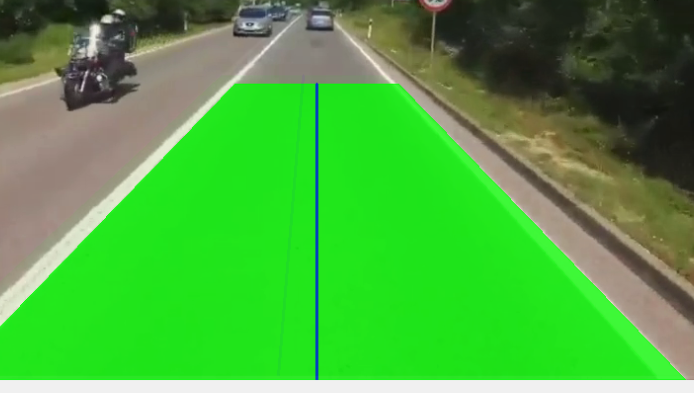
\includegraphics[width=2.5in]{video1_screenshot}
\caption{Screenshot of the solution correctly highlighting the current lane in green}
\label{fig:t5working}
\end{figure}


\subsection{Limitations}\label{sec:t2_lim}
In it's current state, the solution would not be fit for purpose. High-risk applications such as self-driving cars, or anything to do with automotive applications, have very narrow margins of error. Additionally, when undefined behaviour occurs, the consequences can include serious injury up to and including, death.

When testing on the provided video - dashcam footage taken from a road in Crikvenica, Croatia - the solution performs well. However, it is not perfect, and several frames of the video cause the detected area to jump erratically to the other lane. Due to the use of a standard Hough line transform, the system cannot recognise dashed lane demarcations with any significant degree of accuracy. In defence of the solution, it has very limited pre-processing done to the feed, and so could be greatly improved upon. For the level of sophistication, the resulting performance is acceptable; nevertheless, inadequate for real-world applications without further improvement. Testing the solution on alternate datasets, such as dashcam footage acquired off of YouTube\cite{SecondVideo}, showed severe inadequacies in the robustness of the solution.

\begin{figure}[H]
\centering
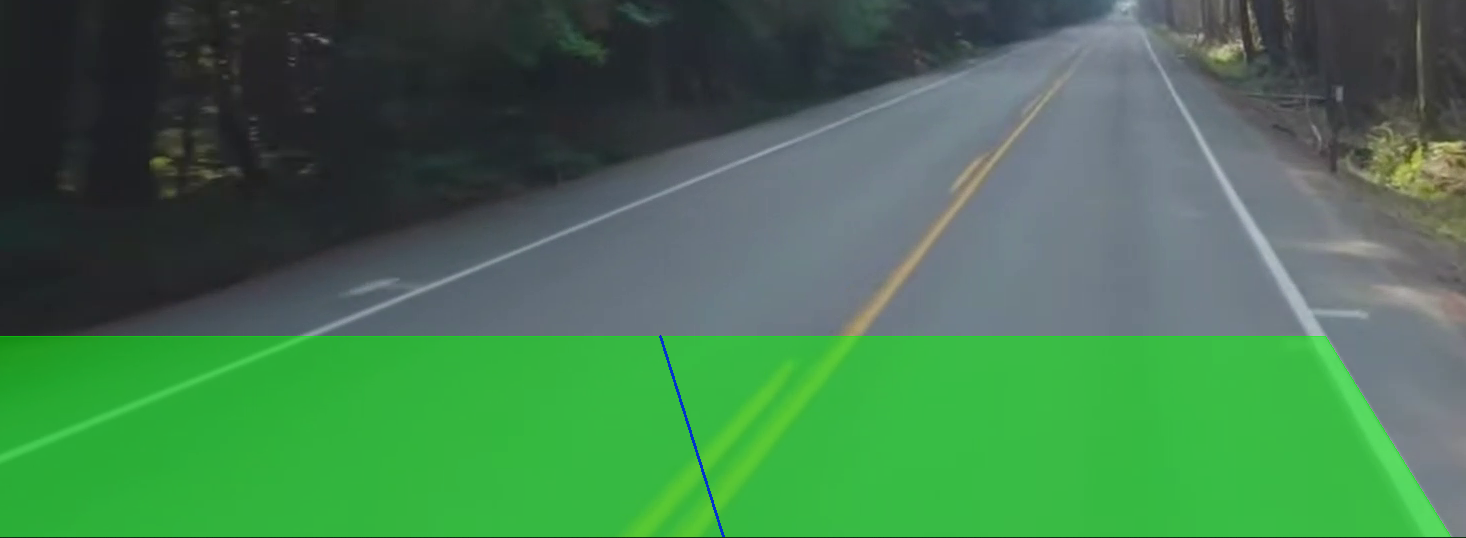
\includegraphics[width=2.5in]{video2_screenshot}
\caption{Screenshot of the solution incorrectly highlighting road markings}
\label{fig:t5working}
\end{figure}

As discussed above, the solution makes use of a standard Hough lines transform. One limitation of the standard transform is that it cannot detect curved lines, and struggles with segmented ones. By switching to a probabilistic Hough lines transform the robustness of the solution could be improved.
\subsection{Further Improvements}
One improvement that could be made is in the noise filtering. While the normalised box filter that \textit{blur} employs is adequate, switching to block-matching and 3D filtering (BM3D) would confer a boost in performance for the edge detection algorithm\cite{Blur}. A cleaner edge map would improve recognition performance throughout the program, and help the solution to deal with less clearly demarcated lanes (such as faded paint, or sub-par lighting conditions.

As discussed in the section prior, the use of standard over probabilistic Hough Line transforms limits the solution's ability to recognise curved and dashed lines. Switching to the probabilistic variant would also have numerous performance benefits, as the probabilistic is more lightweight. Running on desktop hardware, performance is of little concern; however any real-life applications would be limited to portable hardware, and so performance overhead would affect the viability of the solution.

\subsection{Conclusion}
Given the heavy limitations placed on the development of the solution, the performance is as expected, with adequate lane tracking on the provided dataset. Performance degrades quickly on any dataset that is not the sample; nor can the solution cope with changes in line colour or continuity. With drastic improvements to both the pre-processing of the images as well as the edge detection methods, the solution may be improved enough to see use in a real-life application.


% An example of a floating figure using the graphicx package.
% Note that \label must occur AFTER (or within) \caption.
% For figures, \caption should occur after the \includegraphics.
% Note that IEEEtran v1.7 and later has special internal code that
% is designed to preserve the operation of \label within \caption
% even when the captionsoff option is in effect. However, because
% of issues like this, it may be the safest practice to put all your
% \label just after \caption rather than within \caption{}.
%
% Reminder: the "draftcls" or "draftclsnofoot", not "draft", class
% option should be used if it is desired that the figures are to be
% displayed while in draft mode.
%
%\begin{figure}[H]
%\centering
%\includegraphics[width=2.5in]{myfigure}
% where an .eps filename suffix will be assumed under latex, 
% and a .pdf suffix will be assumed for pdflatex; or what has been declared
% via \DeclareGraphicsExtensions.
%\caption{Simulation Results}
%\label{fig_sim}
%\end{figure}

% Note that IEEE typically puts floats only at the top, even when this
% results in a large percentage of a column being occupied by floats.


% An example of a double column floating figure using two subfigures.
% (The subfig.sty package must be loaded for this to work.)
% The subfigure \label commands are set within each subfloat command, the
% \label for the overall figure must come after \caption.
% \hfil must be used as a separator to get equal spacing.
% The subfigure.sty package works much the same way, except \subfigure is
% used instead of \subfloat.
%
%\begin{figure*}[!t]
%\centerline{\subfloat[Case I]\includegraphics[width=2.5in]{subfigcase1}%
%\label{fig_first_case}}
%\hfil
%\subfloat[Case II]{\includegraphics[width=2.5in]{subfigcase2}%
%\label{fig_second_case}}}
%\caption{Simulation results}
%\label{fig_sim}
%\end{figure*}
%
% Note that often IEEE papers with subfigures do not employ subfigure
% captions (using the optional argument to \subfloat), but instead will
% reference/describe all of them (a), (b), etc., within the main caption.


% An example of a floating table. Note that, for IEEE style tables, the 
% \caption command should come BEFORE the table. Table text will default to
% \footnotesize as IEEE normally uses this smaller font for tables.
% The \label must come after \caption as always.
%
%\begin{table}[!t]
%% increase table row spacing, adjust to taste
%\renewcommand{\arraystretch}{1.3}
% if using array.sty, it might be a good idea to tweak the value of
% \extrarowheight as needed to properly center the text within the cells
%\caption{An Example of a Table}
%\label{table_example}
%\centering
%% Some packages, such as MDW tools, offer better commands for making tables
%% than the plain LaTeX2e tabular which is used here.
%\begin{tabular}{|c||c|}
%\hline
%One & Two\\
%\hline
%Three & Four\\
%\hline
%\end{tabular}
%\end{table}


% Note that IEEE does not put floats in the very first column - or typically
% anywhere on the first page for that matter. Also, in-text middle ("here")
% positioning is not used. Most IEEE journals/conferences use top floats
% exclusively. Note that, LaTeX2e, unlike IEEE journals/conferences, places
% footnotes above bottom floats. This can be corrected via the \fnbelowfloat
% command of the stfloats package.

\newpage
\newpage
\appendix

\printbibliography


\onecolumn
\subsection{Github Repository}
For the full code, please see the linked github repository \href{https://github.com/jjpendlebury/AINT308-Coursework}{HERE}.
\subsection{Task 4 Figures}\label{app:T4}
\begin{figure}[H]
\centering
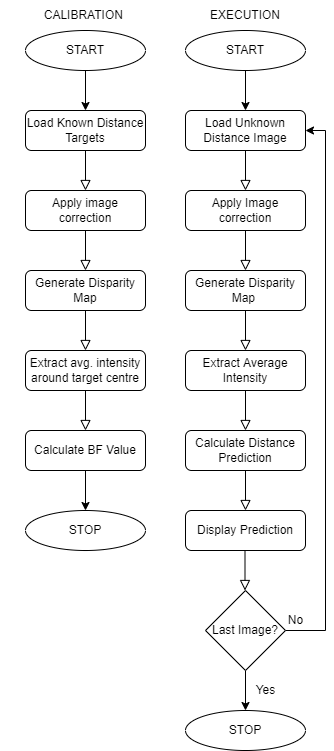
\includegraphics[width=3in]{Task4.drawio}
\caption{Flowchart showing Task 4 solution outline}
\label{fig:flowchart4}
\end{figure}
\begin{table}[H]
\caption{Full results of the intensity testing}
\label{tab:T4_full}
\begin{tabular}{lllll}
\textbf{Distance} & \textbf{Validation} & \textbf{Error} & \textbf{Program Result} & \textbf{Program Error} \\
30                & 29.82616046         & 0.58\%         & 29.8134                 & 0.62\%                 \\
40                & 39.8889162          & 0.28\%         & 39.8747                 & 0.31\%                 \\
50                & 50.14148903         & -0.28\%        & 50.1235                 & -0.25\%                \\
60                & 60.02514793         & -0.04\%        & 60.025                  & -0.04\%                \\
70                & 69.6720467          & 0.47\%         & 69.6632                 & 0.48\%                 \\
80                & 79.72688869         & 0.34\%         & 79.6928                 & 0.38\%                 \\
90                & 88.79964985         & 1.33\%         & 88.7714                 & 1.37\%                 \\
100               & 98.93209801         & 1.07\%         & 98.8448                 & 1.16\%                 \\
110               & 108.3787393         & 1.47\%         & 108.378                 & 1.47\%                 \\
120               & 121.6884091         & -1.41\%        & 121.556                 & -1.30\%                \\
130               & 130.3259997         & -0.25\%        & 130.175                 & -0.13\%                \\
140               & 144.5049858         & -3.22\%        & 144.356                 & -3.11\%                \\
150               & 150.7878112         & -0.53\%        & 150.747                 & -0.50\%               
\end{tabular}
\end{table}
\newpage
\subsection{Task 5 Figures}\label{app:T5}
\begin{figure}[H]
\centering
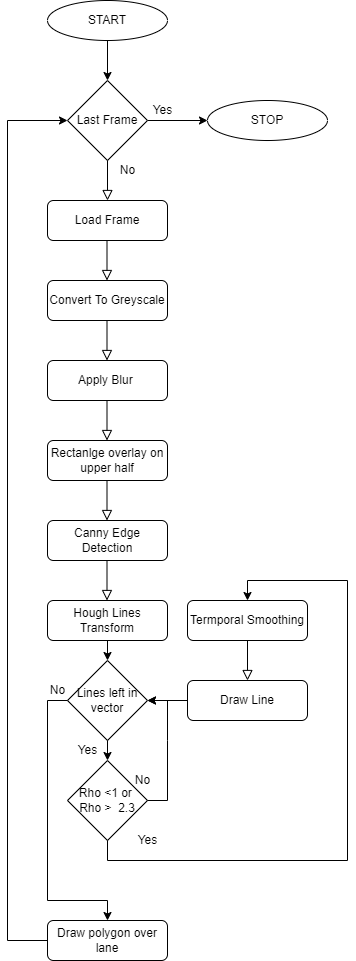
\includegraphics[width=3in]{Task5.drawio}
\caption{Flowchart showing Task 5 solution outline}
\label{fig:flowchart5}
\end{figure}
\subsection{Code Printouts}
The following pages contain complete printouts of the code used to implement the solutions outlined above, for reference.
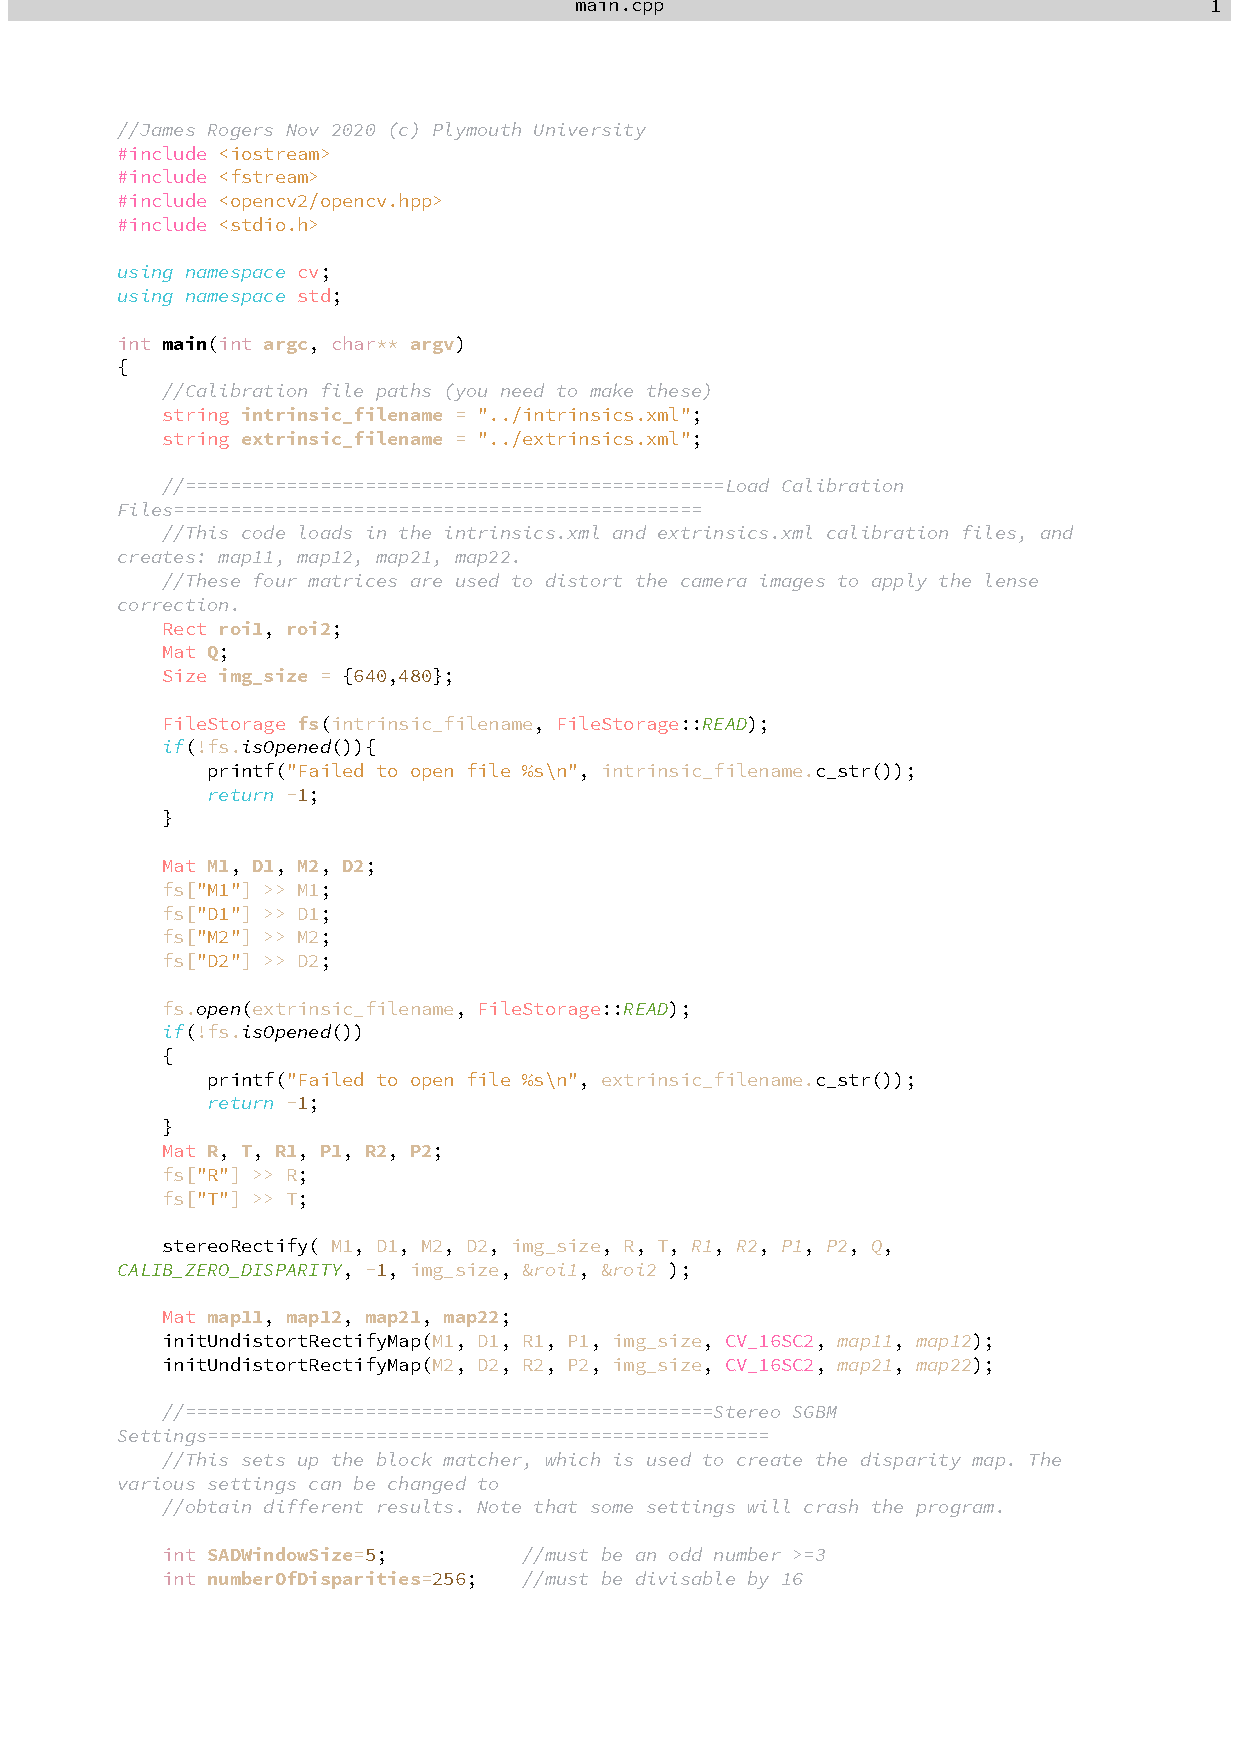
\includepdf[pages=-,offset=0 -50]{Task4.pdf}
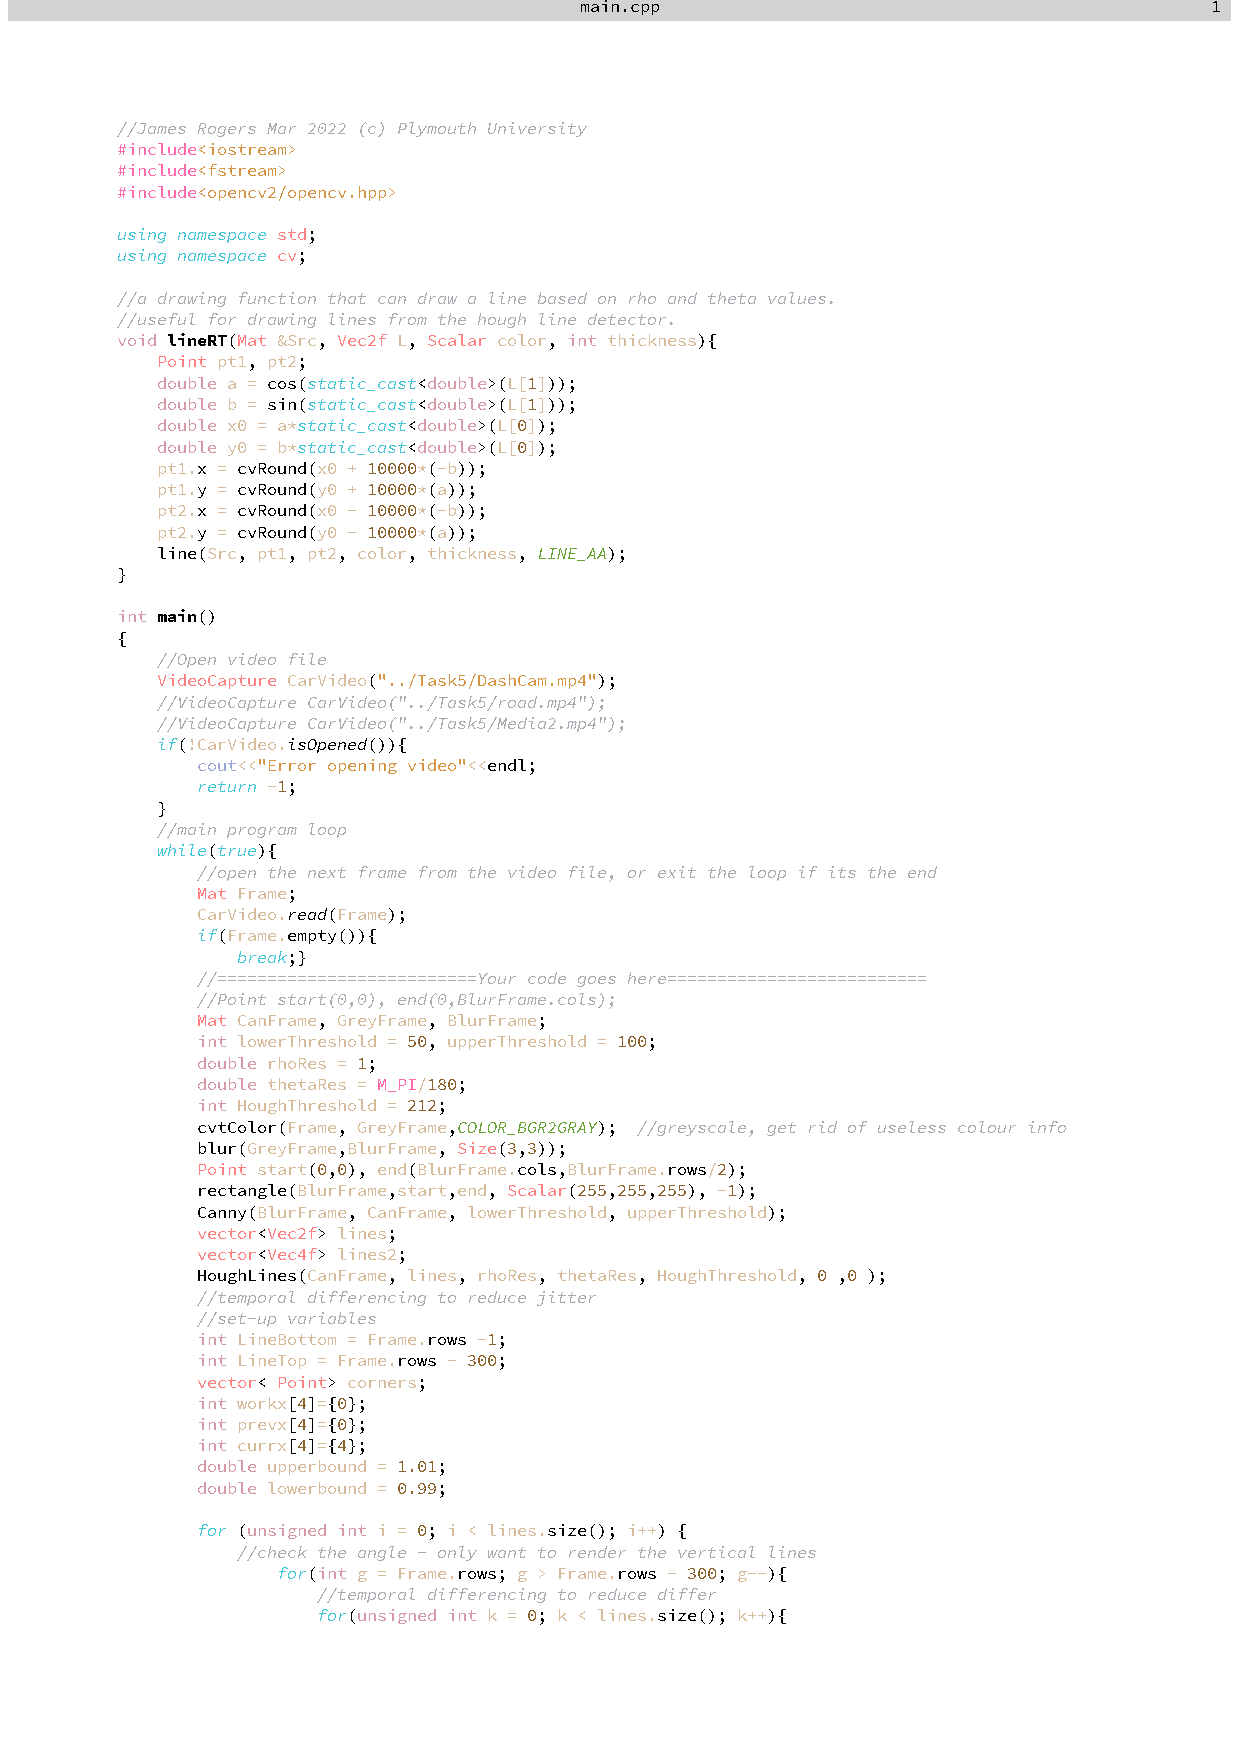
\includepdf[pages=-,offset=0 -50]{Task5.pdf}
%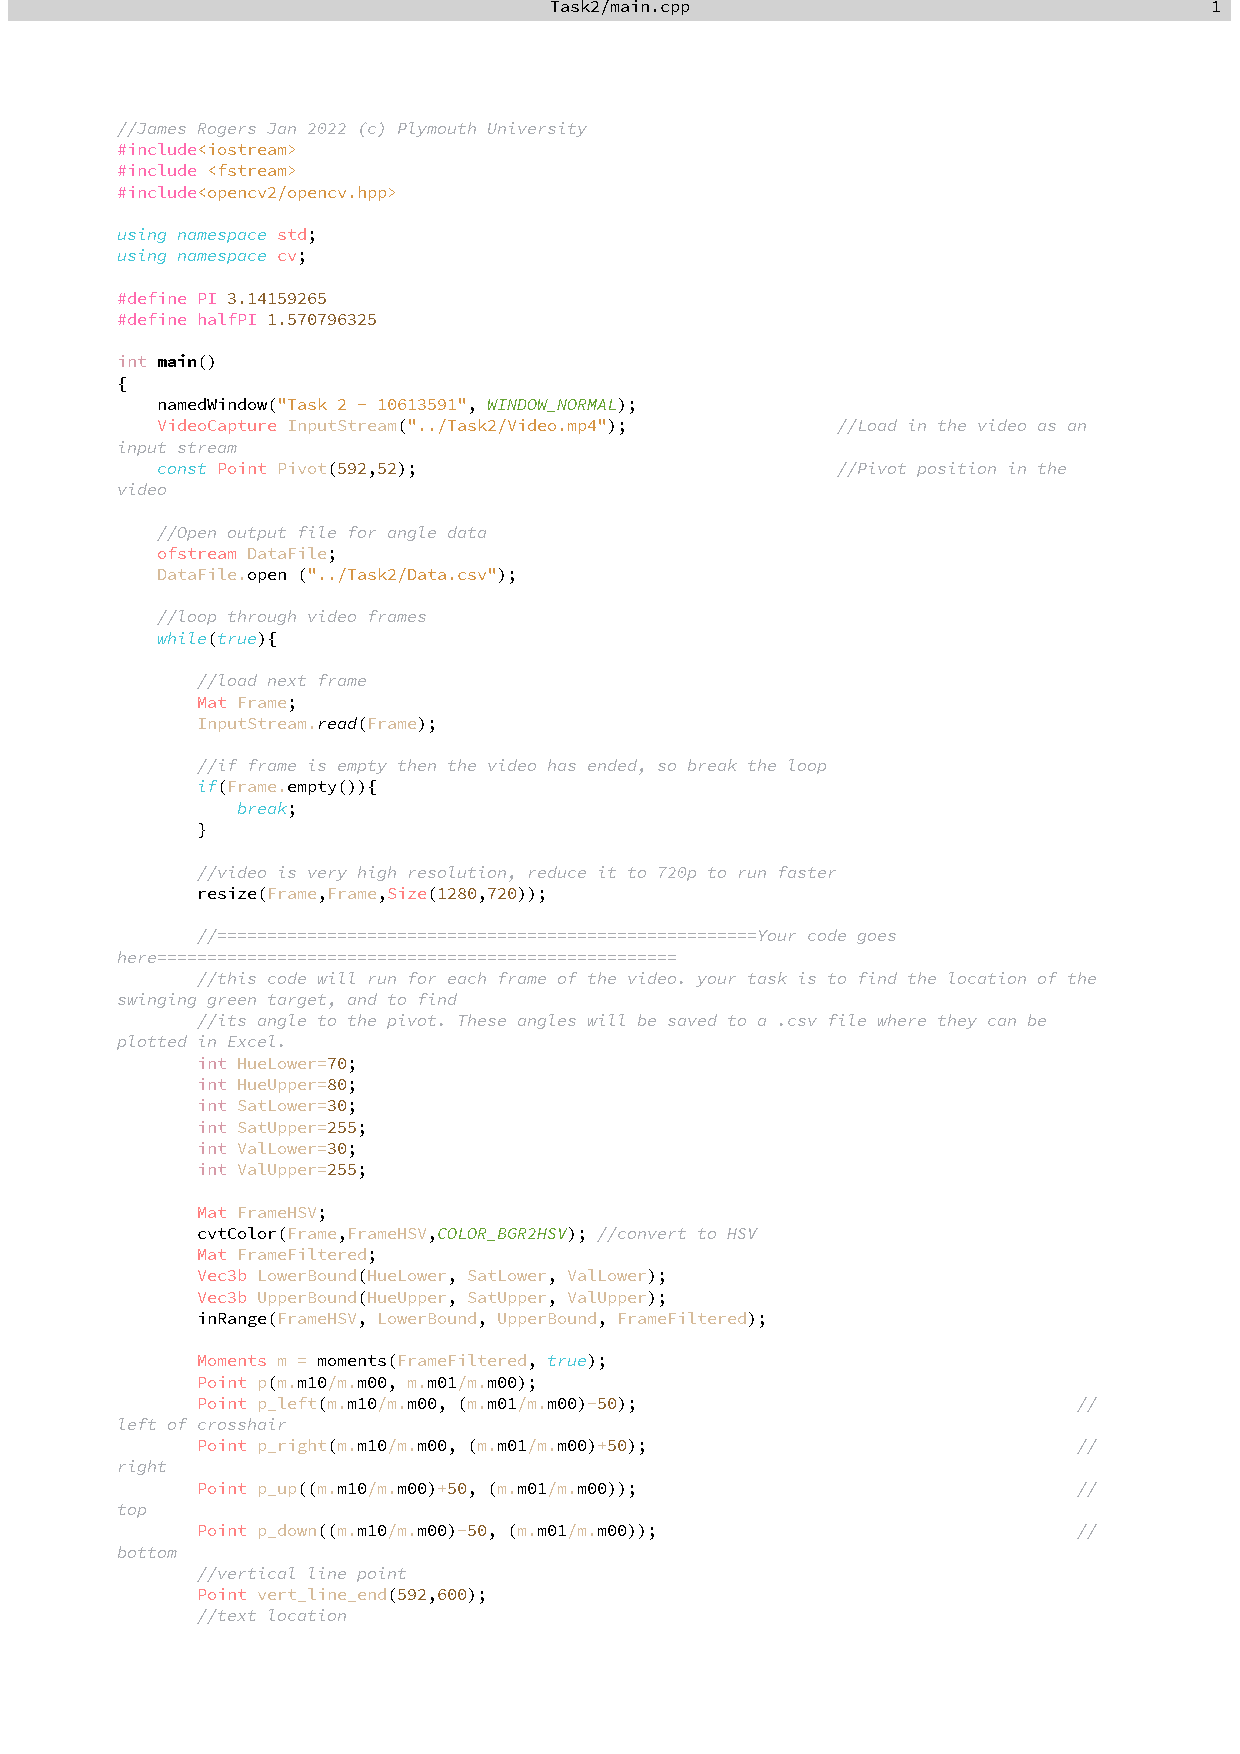
\includepdf[pages=-,offset=0 -50]{task2_code.pdf}
%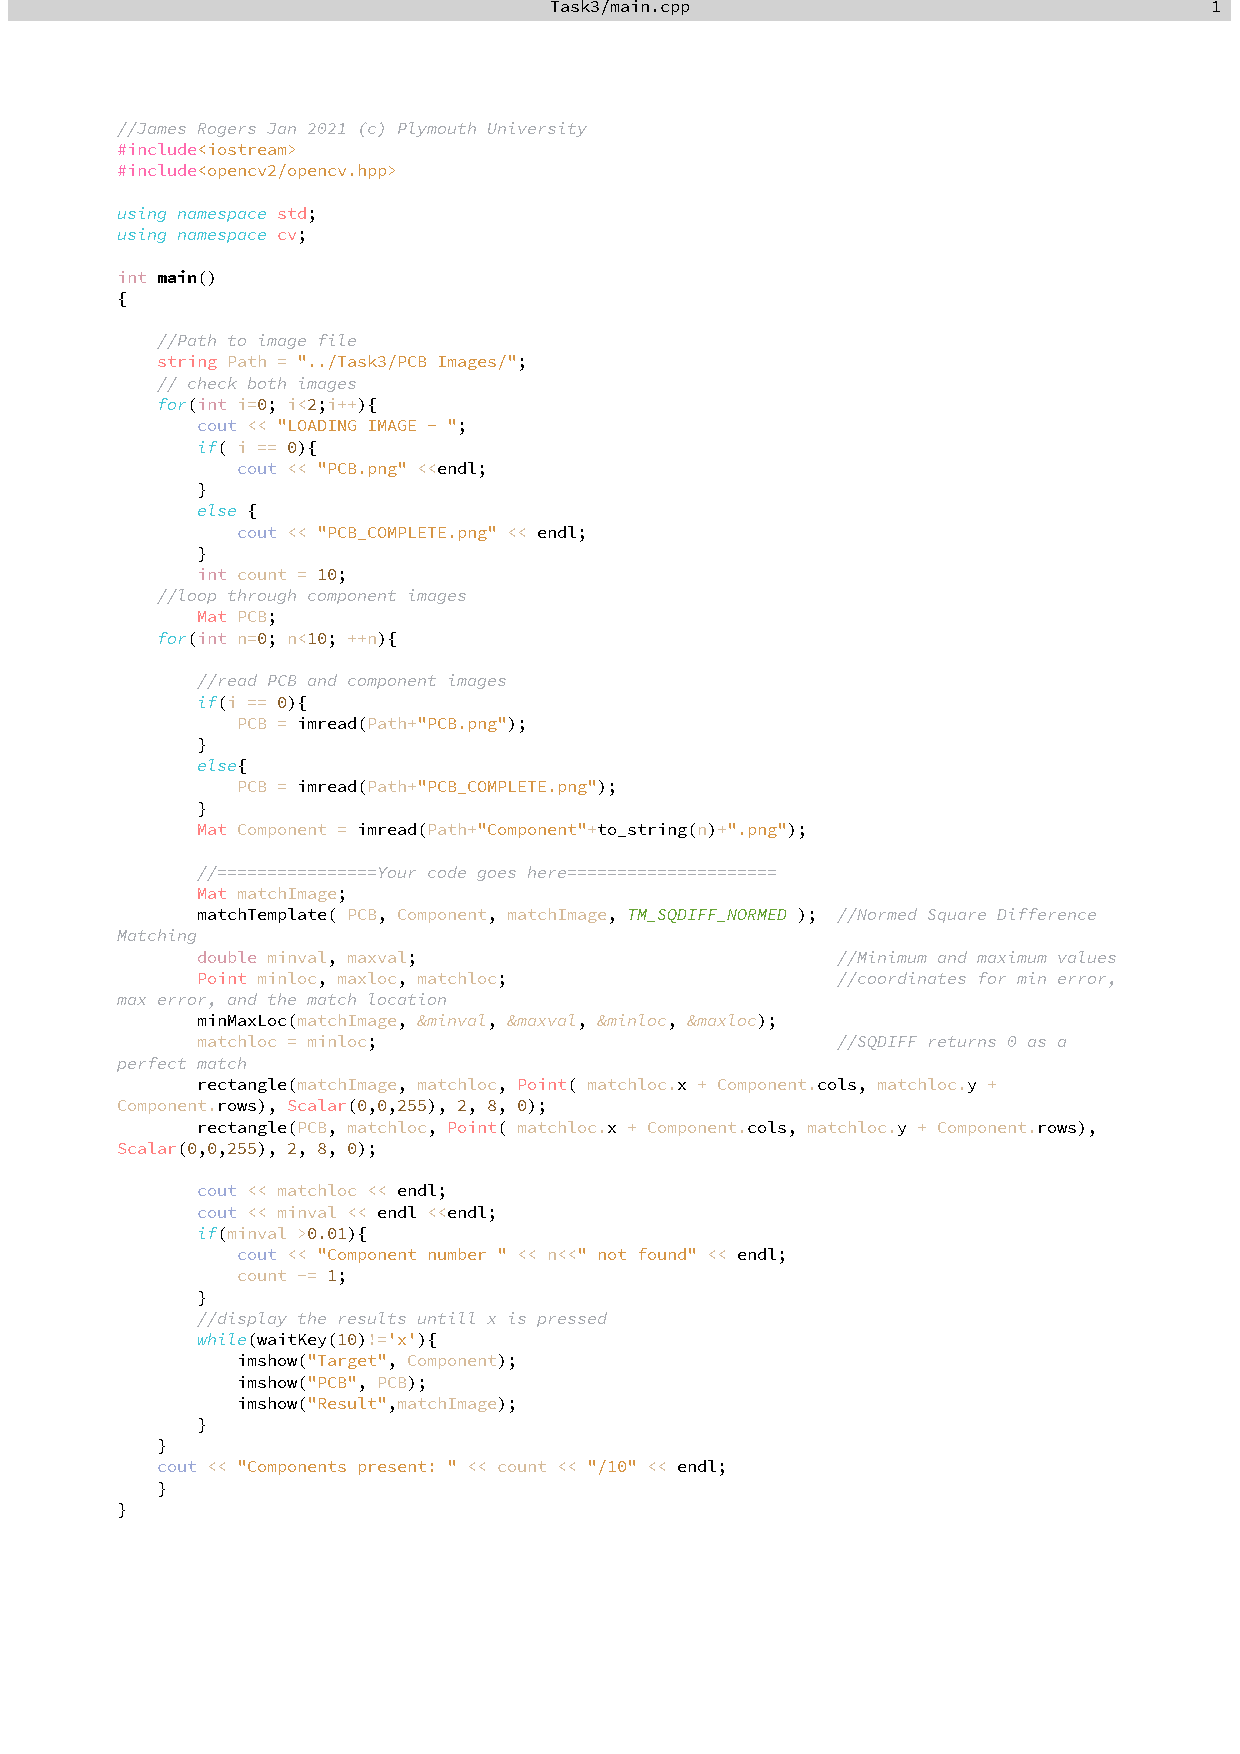
\includepdf[pages=-,offset=0 -50]{task3_code.pdf}
% that's all folks
\end{document}